\documentclass[12pt]{article}
\usepackage[utf8]{inputenc}
\usepackage{graphicx} % Allows you to insert figures
\usepackage{amsmath} % Allows you to do equations
\usepackage{fancyhdr} % Formats the header
\usepackage{geometry} % Formats the paper size, orientation, and margins
\linespread{1.25} % about 1.5 spacing in Word
\setlength{\parindent}{0pt} % no paragraph indents
\setlength{\parskip}{1em} % paragraphs separated by one line
\usepackage[format=plain,
            font=it]{caption} % Italicizes figure captions
\usepackage[english]{babel}
\usepackage{csquotes}
\renewcommand{\headrulewidth}{0pt}
\geometry{letterpaper, portrait, margin=1in}
\setlength{\headheight}{14.49998pt}
\geometry{a4paper, left=20mm, right=20mm, top=35mm, bottom=20mm}

\newcommand\titleofdoc{\textbf{Assignment-6: The Laplace Transform}}
\newcommand\GroupName{EE20B136}

\begin{document}
\begin{titlepage}
   \begin{center}
        \vspace*{4cm} % Adjust spacings to ensure the title page is generally filled with text

        \Huge{\titleofdoc} 

        \vspace{3 cm}
        \Large{Syam SriBalaji T}
       
        \vspace{0.25cm}
        \large{EE20B136}
       
        \vspace{3 cm}
        \Large{March 17, 2022}
        
        \vspace{0.25 cm}
        \Large{EE2703 :Jan-May 2022}
       

       \vfill
    \end{center}
\end{titlepage}

\setcounter{page}{2}
\pagestyle{fancy}
\fancyhf{}
\rhead{\thepage}

\section*{Spring's Time response:}

Here we are going to obtain time response of spring system with the given conditions.\\
On solving in the Laplace domain, we get the following equation\\
\begin{multline}  
F(s)=\frac{s + 0.5}{((s^2 + 0.5)^2 + 2.25)(s^2 + 2.25)}=\frac{s + 0.5}{(s^2 + s + 2.5)(s^2 + 2.25)}\\
\end{multline} 

\begin{figure}[h!]
\centering
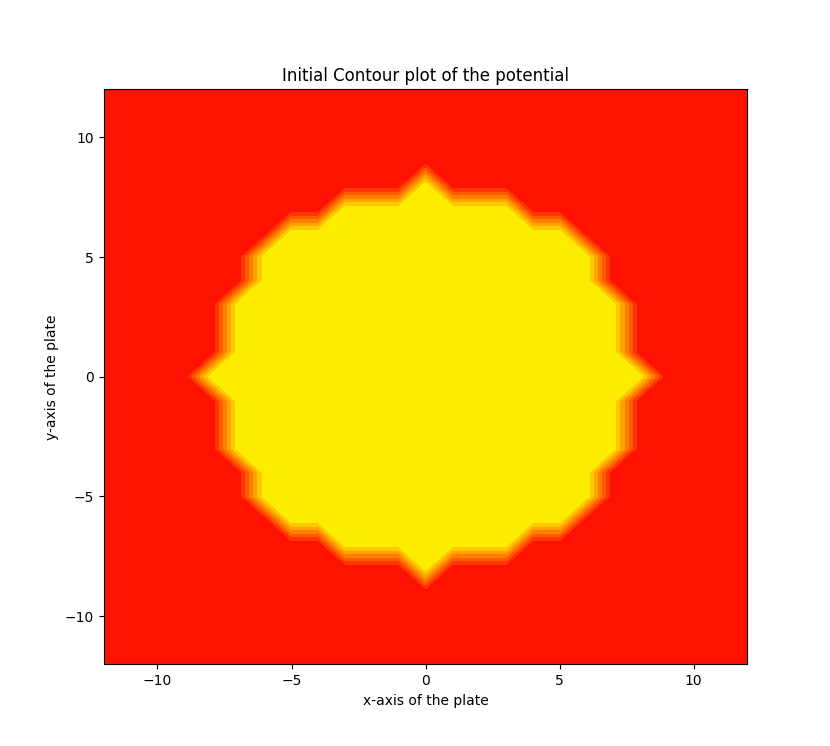
\includegraphics[height=9cm]{Figure_1.png}
\end{figure}

\newpage
\section*{Spring's Time response with smaller decay:}

The same problem above is solved here with smaller decay constant, so we get the following transfer equation\\

\begin{multline}  
F(s)=\frac{s + 0.05}{((s^2 + 0.05)^2 + 2.25)(s^2 + 2.25)}=\frac{s + 0.5}{(s^2 + s + 2.2525)(s^2 + 2.25)}\\
\end{multline}

\begin{figure}[h!]
\centering
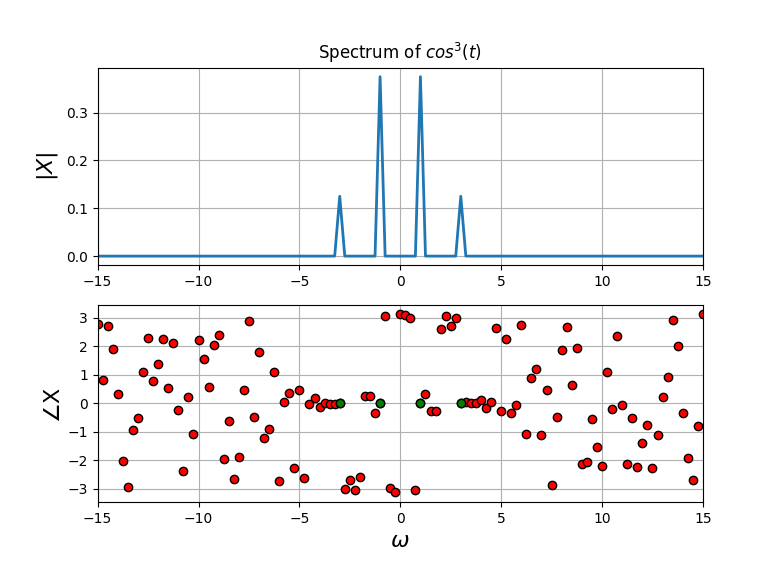
\includegraphics[height=9cm]{Figure_2.png}
\end{figure}

\newpage
\section*{LTI response for different frequencies:}

From the given input, we find resulting responses for different frequency, thus the plots are-\\

\begin{figure}[h!]
\centering
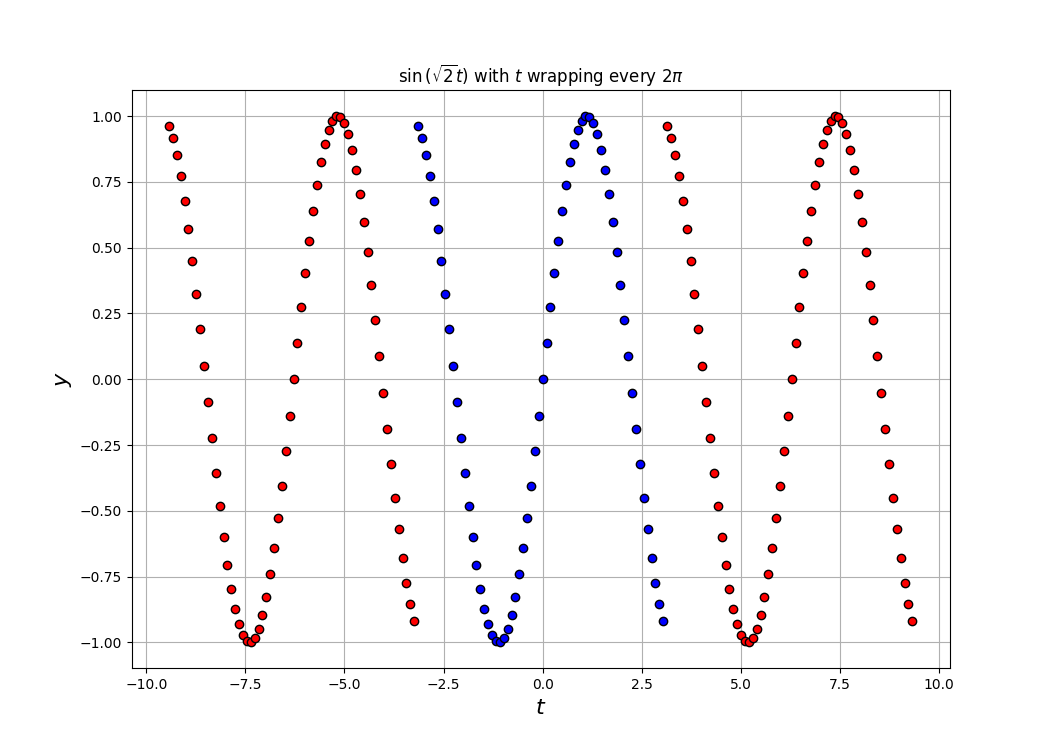
\includegraphics[height=9cm]{Figure_3.png}
\label{fig:exemplo}
\end{figure}

\textbf{Inference:} Here we can clearly notice that, among all the 5 plots, plot with frequency=1.5 (rad/s) is having maximum amplitude.

\newpage
\section*{Time evolution of Coupled Spring problem: }

From the given initial conditions of coupled equations, we get the following transfer function for X and Y in Laplace domain.
\begin{multline}  
\newline X(s)=\frac{s^2 + 2}{s^3 + 3s}
\newline Y(s)=\frac{2}{s^3 + 3s}\\
\end{multline}

\begin{figure}[h!]
\centering
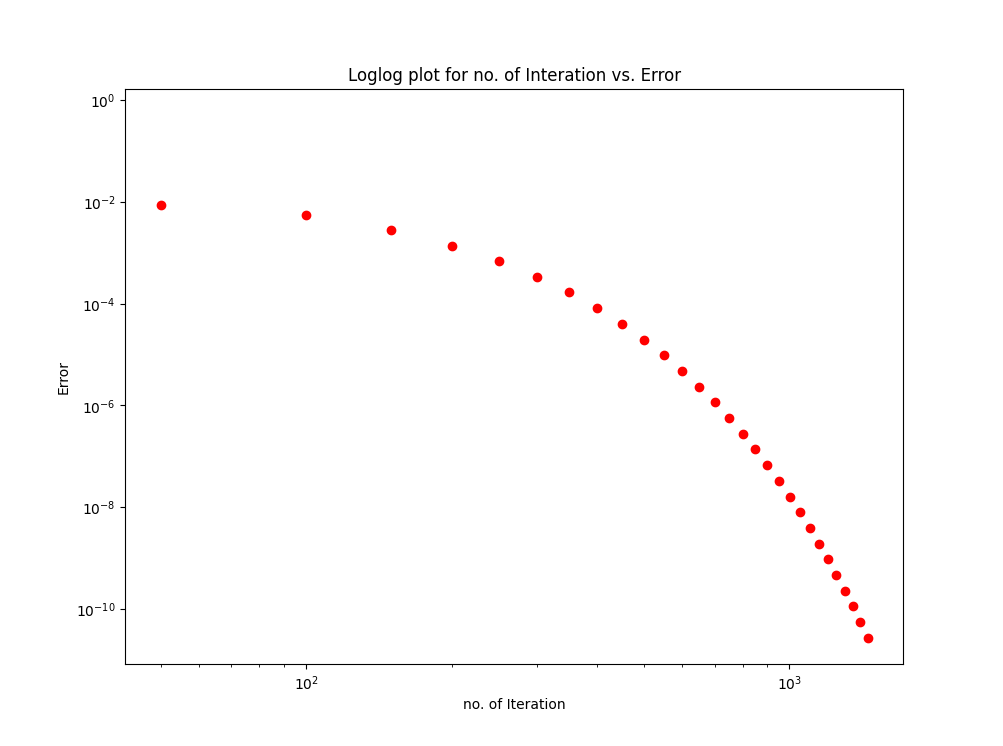
\includegraphics[height=9cm]{Figure_4.png}
\label{fig:exemplo}
\end{figure}

\textbf{Inference:} Here we can notice that plots of Solution of X(t) and Y(t) are sinusoidal with same frequency and phase difference of π. And also their amplitudes are 1 and 1.33 respectively.

\newpage
\section*{Steady state Transfer function of Two-port network:}

Solving the given circuit in Laplace domain, we get the following transfer function-\\


H(s)=\dfrac{10^6}{s^2 + 100s + 10^6} 

Here is the Magnitude and Phase response plots of H(s)-

\begin{figure}[h!]
\centering
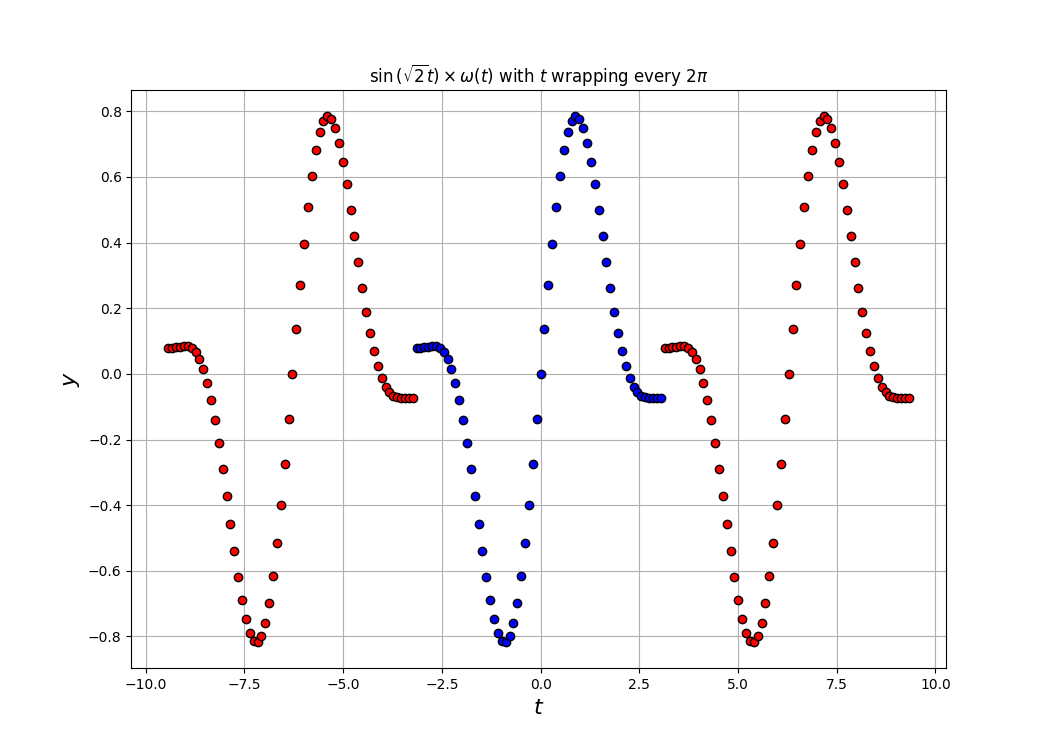
\includegraphics[height=12cm]{Figure_5.png}
\label{fig:exemplo}
\end{figure}
 
\textbf{Inference:} {\sl signal.bode()\/} function can be used to plot this.

\newpage
\section*{Two-port network with a Input signal}

Now, In the same circuit above a input is given to the system,\\
\begin{equation*}
    v_{i}(t)=(cos(10^3t)-cos(10^6t))\times u(t)
\end{equation*}
And the output is 
\begin{equation*}
    v_{o}(s)=v_{i}(s)\times H(s)\\
\end{equation*}
Here we plot 
\begin{equation*}
v_{o}(t) \hspace{0.3cm}in\hspace{0.3cm}  0 < t < 30\mu s\\    
\end{equation*}t


\begin{figure}[h!]
\centering
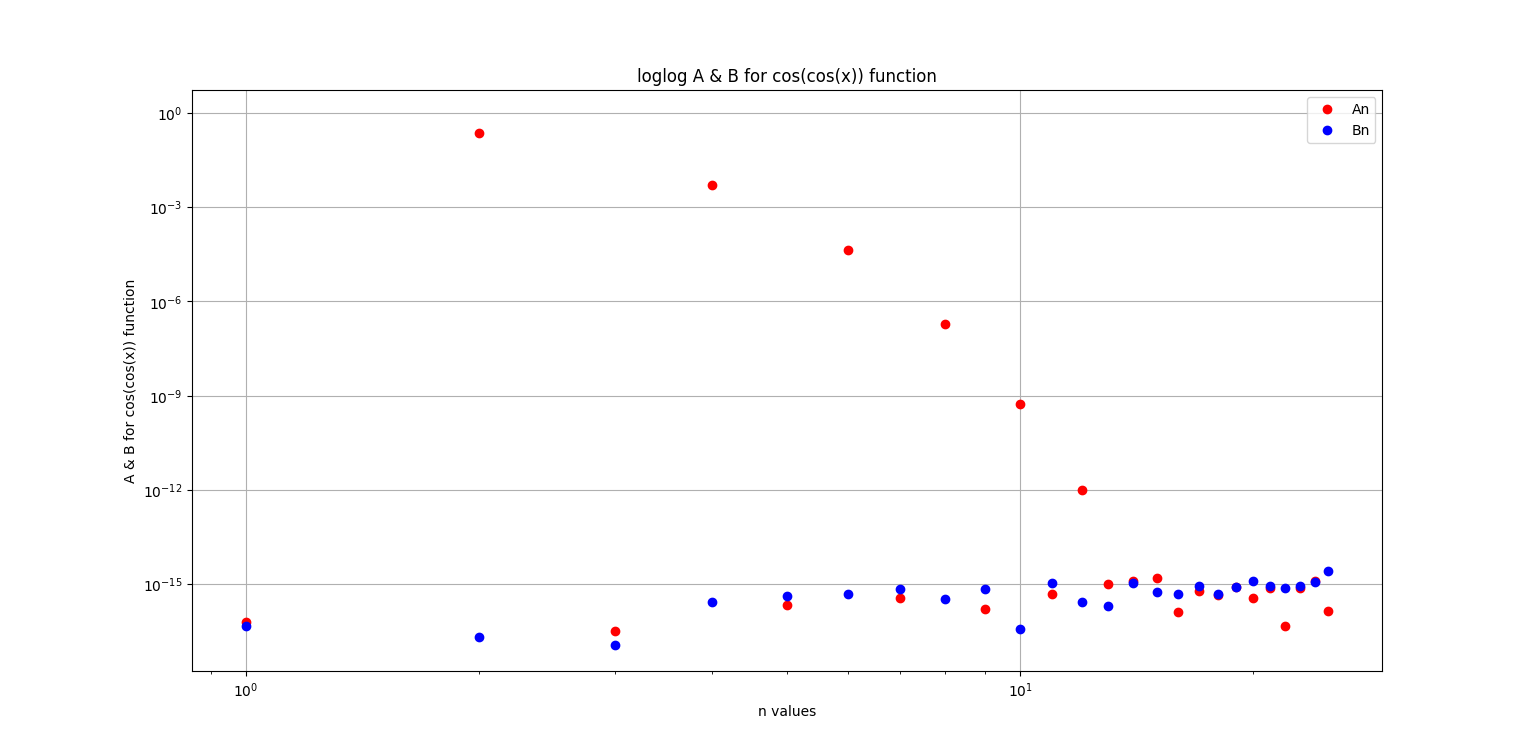
\includegraphics[height=12cm]{Figure_6.png}
\label{fig:exemplo}
\end{figure}

\textbf{Inference:} {\sl lsim function from scipy.signal\/} can be used in this plot.

\newpage
Same as the above question, here that Bode plot is drawn with higher frequency and different range i.e. $0 < t < 10ms$. And also with the given conditions, we get the following plot-

\begin{figure}[h!]
\centering
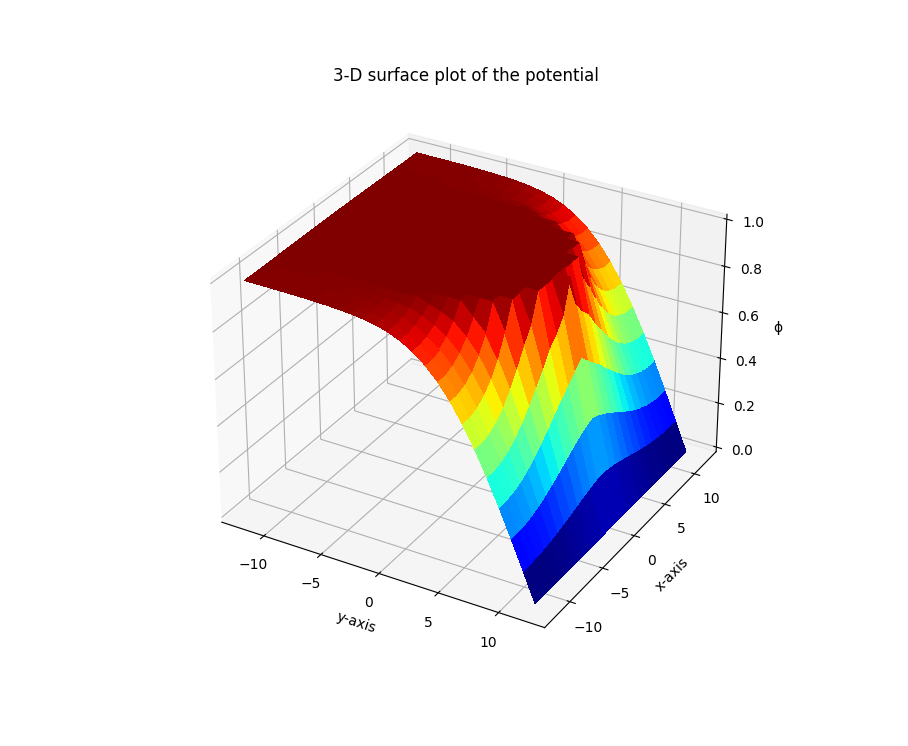
\includegraphics[height=10cm]{Figure_7.png}
\label{fig:exemplo}
\end{figure}



\textbf{Inference:} {\sl lsim function from scipy.signal\/} can be used in this kind of plots.\\
From the Bode plot of H(s), we can notice that the system provides unity gain for a low frequency of 10^3 rad/s.\\
$However, the system dampens a high frequency of 10^6 rad/s, with \hspace{0.4cm}|H(s)|_{dB} \approx −40 .$\\\\
And also from the given circuit we find that it is a Low pass filter. Thus, magnitude of
oscillations of these frequency is reduced.

\begin{center} 
\textbf{Thank you!}
\end{center} 
\end{document}
